\documentclass{Latex_Euclid_style}

%\@ifundefined{textcolor}{}
%{%
% \definecolor{BLACK}{gray}{0}
% \definecolor{WHITE}{gray}{1}
% \definecolor{RED}{rgb}{1,0,0}
% \definecolor{GREEN}{rgb}{0,1,0}
% \definecolor{BLUE}{rgb}{0,0,1}
% \definecolor{CYAN}{cmyk}{1,0,0,0}
% \definecolor{MAGENTA}{cmyk}{0,1,0,0}
% \definecolor{YELLOW}{cmyk}{0,0,1,0}
% }

%%%%%%%%%%%%%%%%%%%%%%%%%%%%%% User specified LaTeX commands.
%\def\citep{\cite}
\def\aap{A\&A}
\def\apj{ApJ}
\def\aapr{A\&A Rev.}
\def\apjl{ApJ}
\def\mnras{MNRAS}
\def\araa{ARA\&A}
\def\aj{AJ}
\def\qjras{QJRAS}
\def\physrep{Phys. Rep.}
\def\nat{Nature}
\def\aaps{A\&A Supp.}
\def\apss{Ap\&SS}      % Astrophysics and Space Science
\def\apjs{ApJS}
\def\prd{Phys. Rev. D}
%%%%%%%%%%%%%%%%%%%%%%%%%%%%%% User specified LaTeX commands.

\usepackage{amsmath}
\usepackage{amsfonts}
\usepackage{amssymb}
\usepackage{graphicx}
\usepackage{epsfig}
\usepackage{psfig}
%\usepackage[numbers,sort&compress]{natbib}
%\usepackage{natbib}
%\usepackage{hyperref}

%\usepackage[numbers,sort&compress]{natbib}
%\usepackage[square,sort,comma,numbers]{natbib}
%\usepackage[nonamebreak]{natbib} 
%\usepackage{hyperref}
%\hypersetup{breaklinks,colorlinks,citecolor=blue}

\usepackage[hang,small,bf]{caption}
\usepackage{rotating}
\usepackage{url}
\usepackage{times}
\usepackage{color}
\usepackage[alsoload=hep]{siunitx}
%\usepackage{babel}
\usepackage{enumitem}
\usepackage{verbatim}
%\usepackage{hyperref}
%\usepackage{ifthen}
%\hypersetup{breaklinks,colorlinks,citecolor=blue}

%%%%%% SP: modified to possibly use the font to Arial (Times New Roman)
%\usepackage[scaled]{uarial}
%\usepackage{times}
%\renewcommand{\familydefault}{\sfdefault}
%\usepackage[T1]{fontenc}
%%%%%%%%%%%%%%%%%%%%%%%%%%%%%%%%%%%%%%%%%%%%%%%%%%%%%%%




\definecolor{orange}{rgb}{1,0.5,0}
\definecolor{darkorange}{rgb}{0.69,0.33,0.13}
\definecolor{fidcol}{rgb}{0.7,0,0}
\newcommand{\CSC}[1]{{\color{darkorange} {\tt {\bf  [CS: #1]}}}}
\newcommand{\mkr}[1]{{\color{blue}\tt [MK: #1]}}
\newcommand{\mk}[1]{{\color{blue}\tt [Martin K: #1]}}
\newcommand{\tk}[1]{{\color{blue}\tt [Tom K: #1]}}
\newcommand{\avr}[1]{{\color{green}\tt [AV: #1]}}
\newcommand{\emr}[1]{{\color{orange}\tt [EM: #1]}}
\newcommand{\com}[1]{{\color{red}\tt [To do: #1]}}
\newcommand{\lavi}[1]{{\color{orange}\tt [lavi: #1]}}
\newcommand{\fid}[1]{{\bf\color{fidcol} #1}}
\newcommand{\cjm}[1]{{\color{blue}\tt [CJM: #1]}}
% --------------

\DeclareSIPrePower\quartic{4}   % declares quartic power for SI units package

\newcommand{\phih}{\ensuremath{\hat{\phi}}}
\newcommand{\phib}{\ensuremath{\bar{\phi}}}
\newcommand{\grad}{\ensuremath{\vec{\nabla}}}
\newcommand{\lap}{\ensuremath{\Delta}}
\newcommand{\adotoa}{\ensuremath{{\cal H}}}
\newcommand{\tadotoa}{\ensuremath{{\cal \tilde{H}}}}
\def\R{{\cal R}}
\def\T{{\cal T}}
\def\L{{\cal L}}
\def\G{{\cal G}}
\def\g{\gamma}
\def\mn{{\mu\nu}}
\def\ij{{ij}}
\def\ab{{ab}}
\def\AB{{AB}}
\def\TT{\tilde{T}}
\def\half{\frac{1}{2}}
\def\quarter{\frac{1}{4}}
\def\del{\partial}
\def\Mpl{M_{\rm pl}}
\newcommand{\FT}{{\cal F}_T}
\newcommand{\GT}{{\cal G}_T}
\newcommand{\e}{{\cal E}}
\newcommand{\p}{{\cal P}}
% --------------

\newcommand{\be}{\begin{equation}}
\newcommand{\ee}{\end{equation}}
\newcommand{\bea}{\begin{eqnarray}}
\newcommand{\eea}{\end{eqnarray}}
\newcommand{\pp}{~~~.}
\newcommand{\vv}{~~~,}
\newcommand{\dd}{\mbox{d}}

\newcommand{\fourier}{\tilde}


\def\rmd{{\rm d}}
\def\comment#1{\textcolor{red}{#1}}
\def\revtext#1{\textcolor{blue}{#1}}
\def\revt#1{\textcolor{red}{#1}}

\begin{document}

\DocTitle{{\bf \emph{Euclid Theoretical Predictions Specification Document (TPSD)}}}
\DocAuths{This document is under the custodianship of the Euclid Inter-Science Working Group 
Taskforce for Forecasting.}
\DocRespb{TWG}
\DocNumbr{EC-???-???}
\DocIssue{0}

\DocAbstr{This document contains the specification of the remit of the inter-science working group taskforce for 
  forecasting and probe combination. Details of how this group relates to the SWGs is defined in the PPSAID.}

\DocDate{\today}

\DocChange{Draft 0 & 0 & 2015-09 & Creation \\ \hline}

\DocApprov{ &  & & \\ \hline}

%\DocHeadr

\header{\DocHeadr}

\mktitlepage

\newpage

\mksecondpage

\newpage

\tableofcontents

\newpage
%\documentclass{Latex_Euclid_style}

%\usepackage{amsmath}
%\usepackage{amsfonts}
%\usepackage{amssymb}
%\usepackage{graphicx}
%\usepackage{epsfig}
%\usepackage[hang,small,bf]{caption}
%\usepackage{rotating}


% --------------

%\begin{document}

\section{Aim}
This document aims at responding to the general need of a common forecasting pipeline, developed in agreement with all SWGs. 
It outlines the approaches that Euclid cosmological parameter forecasting will take during the 
implementation phase (2015--) and up until launch. This will cover standard `Fisher' forecasting methodology, 
as well as more complex predictions. Specifications for the primary probe forecasts are defined, as well 
as how these should be combined together and with external cosmological parameter constraints, in particular 
CMB data. This document will also define the general code infrastructure that the forecasting pipeline will 
use, in preparation for the theoretical calculations that will enter into the Euclid likelihood pipeline 
(that will take output from the SGS LE3, and theoretical computations outlined here). 

Therefore this document covers:
\begin{enumerate}
\item Definition of the primary probe theoretical computation data flow
\item The specification of code comparisons at each stage of the data flow -- in building a single common pipeline
\item Specifications for code comparison for existing non-trunk or external forecast codes
\item How to compare Fisher matrices for a minimal Fisher matrix code 
\item Definition of coding practices -- including language, licensing and publication policy when using IST products etc. 
\item How the code interacts with the SGS 
\item How to deal with new input provided by the SWGs (for example if there is a new parameter 
  or a new forecasting method developed by the SWG, how does the IST react). 
\end{enumerate}

\section*{Applicable Documents} 
\begin{itemize} 
\item 
PPSAID (Post Processing Science Analysis Implementation Document) 
\item 
Theory Parameter Defintion Document 
\item 
SGS Data Flow Down Description Data 
\item 
GDPRD (Ground Data Processing Requirements Document)
\item 
OU RSDs (Requirement Specification Documents)
\item 
MPD (Mission Performance Document) 
\end{itemize} 

\section{Relation to the Euclid Likelihood Pipeline} 
This document describes how the \emph{theoretical} calculations for the Euclid primary probes are made. 
These calculations are initially, before launch, to be used to create Euclid `forecasts'. A forecast 
is a performance prediction for Euclid that makes a statement about the accuracy and precision that Euclid 
will be able to achieve the Level 0 objectives outlines in the Mission Performance Document (MPD). 
This document also describes how the primary probes will be combined. 

The construction of the Euclid likelihood pipeline is described conceptually in the PPSAID. This describes how there 
are three elements that need to come together in order for Euclid to achieve its science objectives. These are 
1) The output from SGS LE3 - i.e. statistics computed on the data, 2) Output from the cosmological simulations 
Science Working Group - who will create realisations of Universe that can be used to create cosmology-dependent 
covariance estimates, and predictions for matter clustering, 3) Predictions of the measured statistics 
from theories against which the data can be tested (i.e. ``forecasts'' before launch).
\begin{figure}
    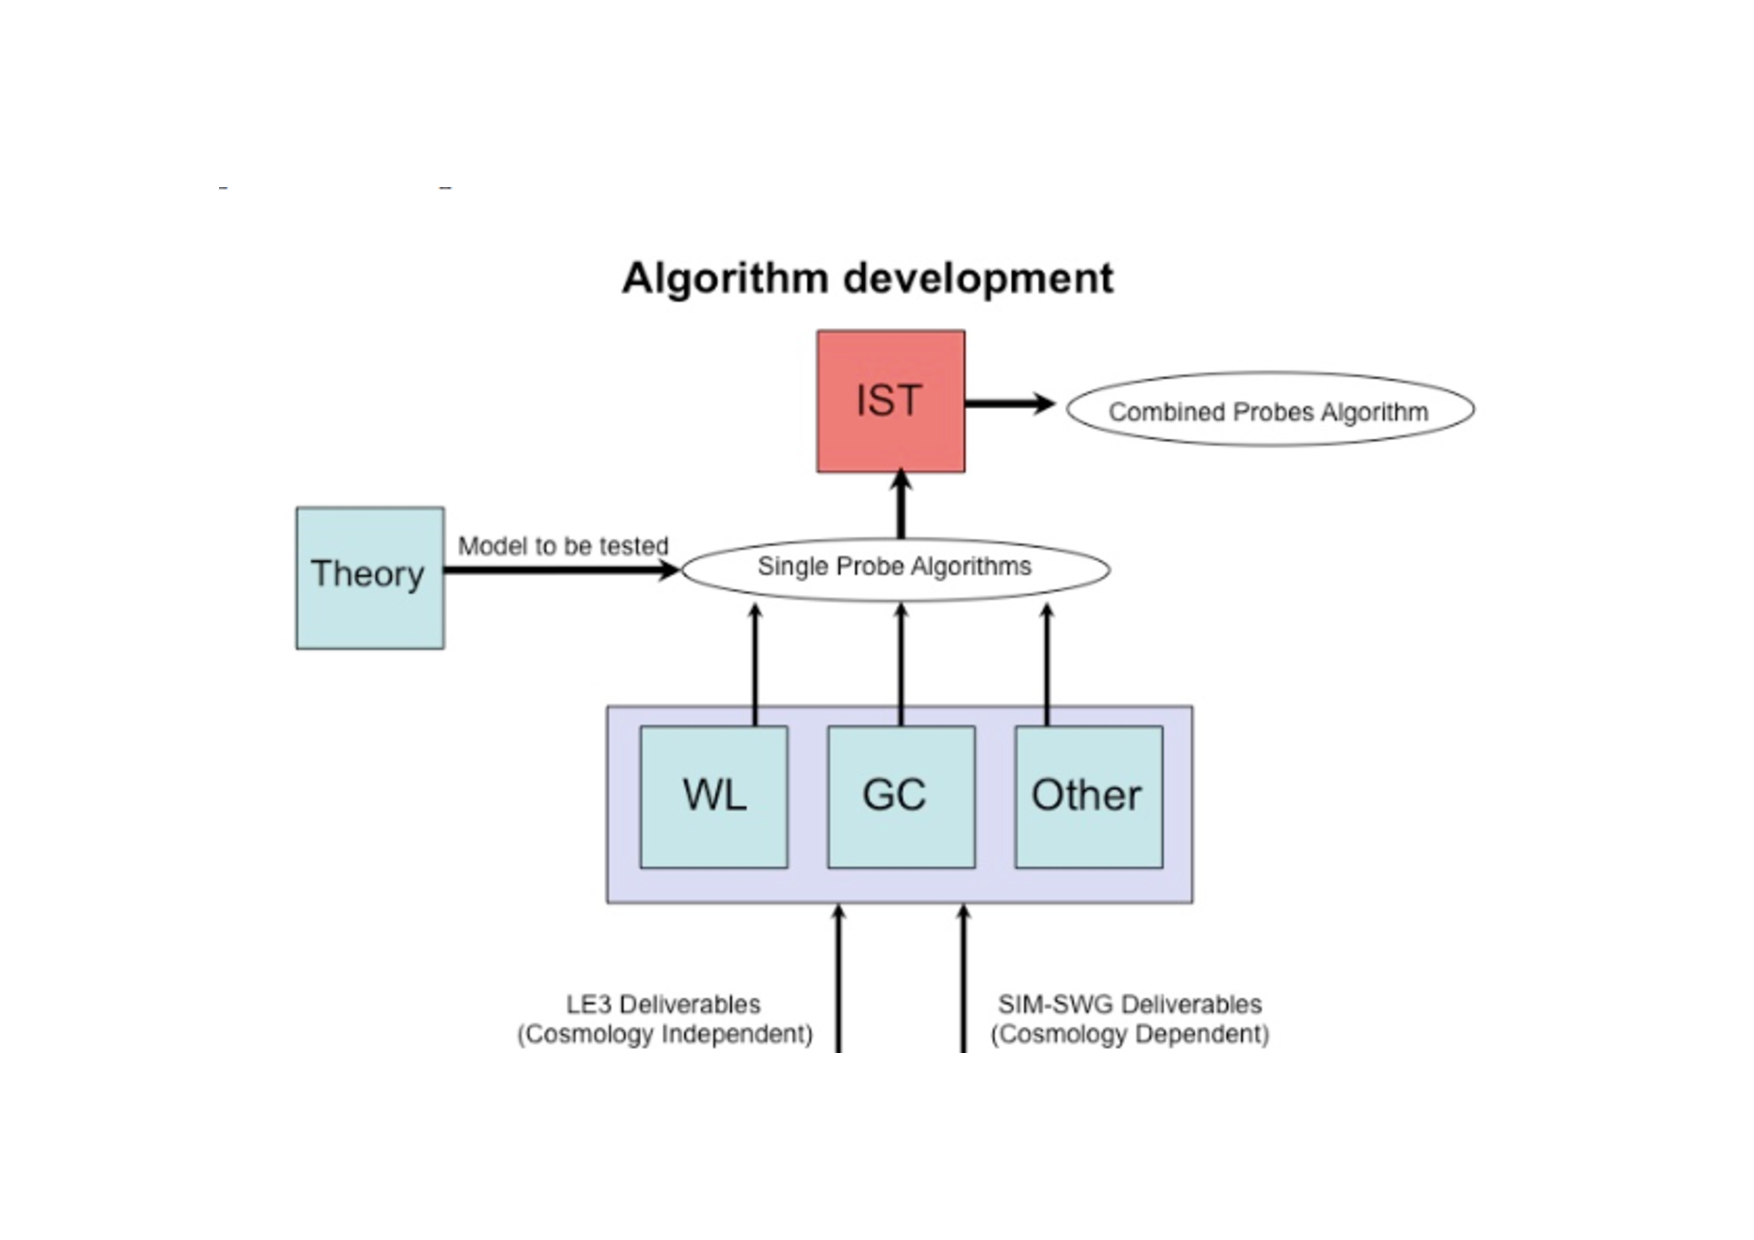
\includegraphics[angle=0,clip=,width=\columnwidth]{ppsaid.pdf}
 \caption{Figure from PPSAID. A schematic of the flow of information to create the algorithms for the individual probes and the combined probes. Note that the development of the algorithms is a collaborative effort between the cosmology SWGs and SGS.}
 \label{ppsaid}
\end{figure}

% SGS 
The theory contruction formally does not involve the SGS algorithm development, but will be constructed such that the 
outputs from the SGS LE3 will be inputs into a likelihood pipeline that will also take inputs from the 
cosmological simulations and input from the theoretical algorithms. This relationship is show in Figure \ref{likelihood}.
\begin{figure}
    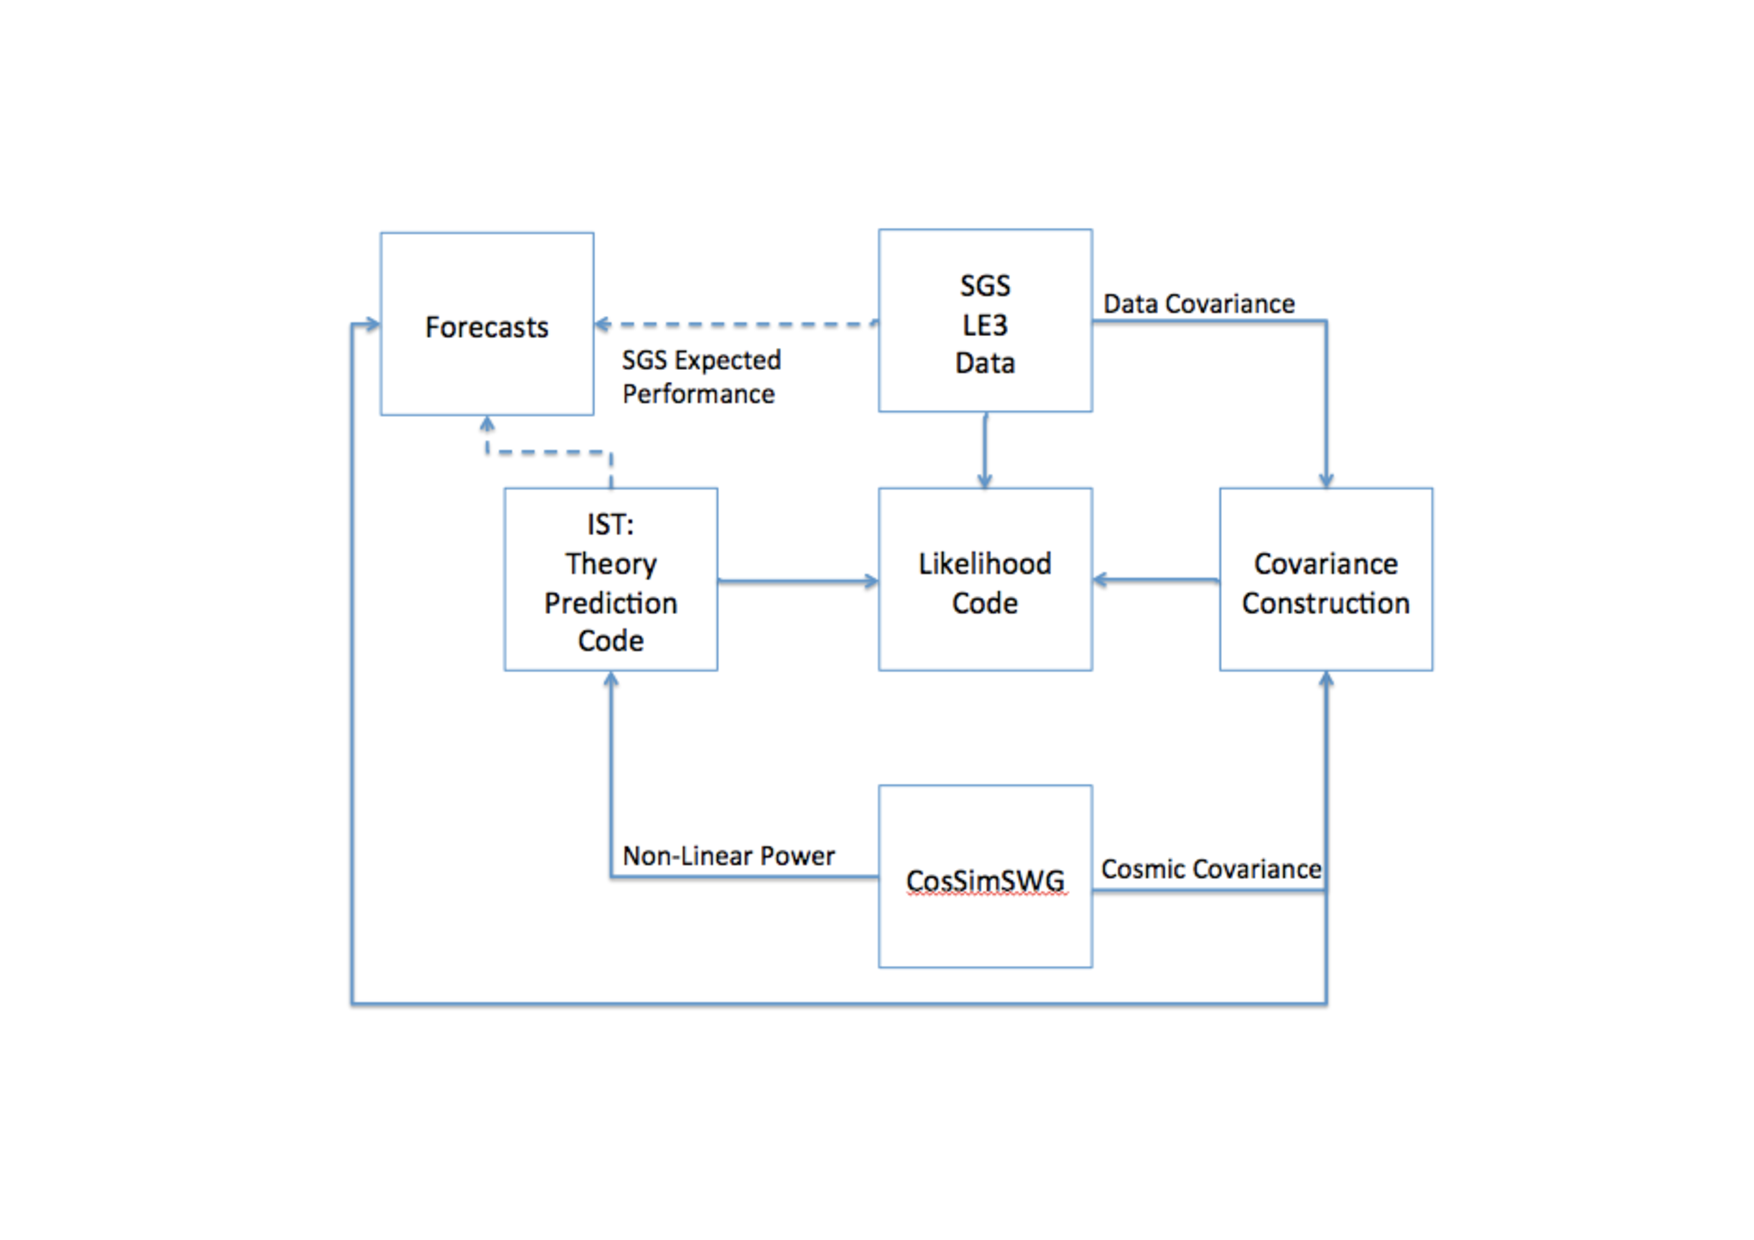
\includegraphics[angle=0,clip=,width=\columnwidth]{likelihood.pdf}
 \caption{How the theory calculations relate to the SGS, CosmoSIMSWG and Euclid likelihood codes. The IST makes theoretical predictions that are incorporated into both forecasts and ultimately into likelihoods.}
 \label{likelihood}
\end{figure}

\section{Definition of Cosmological Statistic Theory-Flows} 
The first step in creating the Euclid forecasting pipeline is to define the data-flow from cosmological parameters, 
and input survey characteristics, to theoretical predictions of relevant statistics. This is a similar procedure to that 
used in the Euclid ground segment to define the data-flow from pixels and spectro-photometry to Level-3 products. We 
adopt a very similar procedure here except that we refer to this as a theory-flow to demark it from SGS activities. 
The statistics, i.e. `observables', that we will use as the primary probe are 
\begin{itemize} 
\item 
The weak lensing tomographic power spectrum 
\item 
Galaxy clustering: BAO, RSD, P(k)
\item 
Secondary cosmological probes: Supernovae, clusters, ... 
\item 
{\bf discussion point: do we need more e.g. 2nd-priority tiers for LE3, i.e. spherical-Bessel stats from the beginning} 
\item
{\bf discussion point: observables may change with the model: ex. isotropy tests may want different $\ell$ requirements.}
\end{itemize} 

In the following we will define a theory-flow down for each of these primary probe statistics, and also for the 
combination of the primary probes, and the combination with CMB data. In doing this 
each element in the theory-flow will be referred to as a ``{\bf Processing Function (PF)}'' using exactly the same 
naming convention as in the SGS for algorithm entities. 

The broad grouping of the processing functions are into
\begin{itemize}
\item 
Inputs: Model and parameter definitions, including cosmological mode and parameters, and nuisance parameters. 
\item 
Inputs: Survey characteristics, including (expected) distributions of observed quantities, and survey geometry.
\item 
Internal: Functions that act internally to the flow, for example matter power spectrum estimatation. 
\item 
Output: These are the expected theoretical statistics, and manipulations of those statistics e.g. derivatives, Fisher matrices etc. 
\end{itemize} 
Each processing function is given a unique identifier that refers to the pipeline(s) in which it is embedded, the nature 
of the processing function, and a short descriptor of its function. 

Finally each theory-flow is required to have a matching data-flow in the SGS documentation i.e. that it is expected that 
the statistics that the theory-flow will compute from a theoretical side will also be computed by the SGS 
from the data for eventual inclusion in a Euclid likelihood pipeline. In the event that this document identifies 
missing data-flows then this should be discussed with the SWG leads, and SGS PO. 

\subsection{Weak Lensing: Tomographic Weak Lensing Theory-Flow}
%example of the WL flow
Here we specify the theory-flow for the tomographic weak lensing. In Figure \ref{WLtomo} we show the flowdown from 
cosmological parameters, nuisance and survey parameters to output statistics and Fisher matrices. 
\begin{figure}
    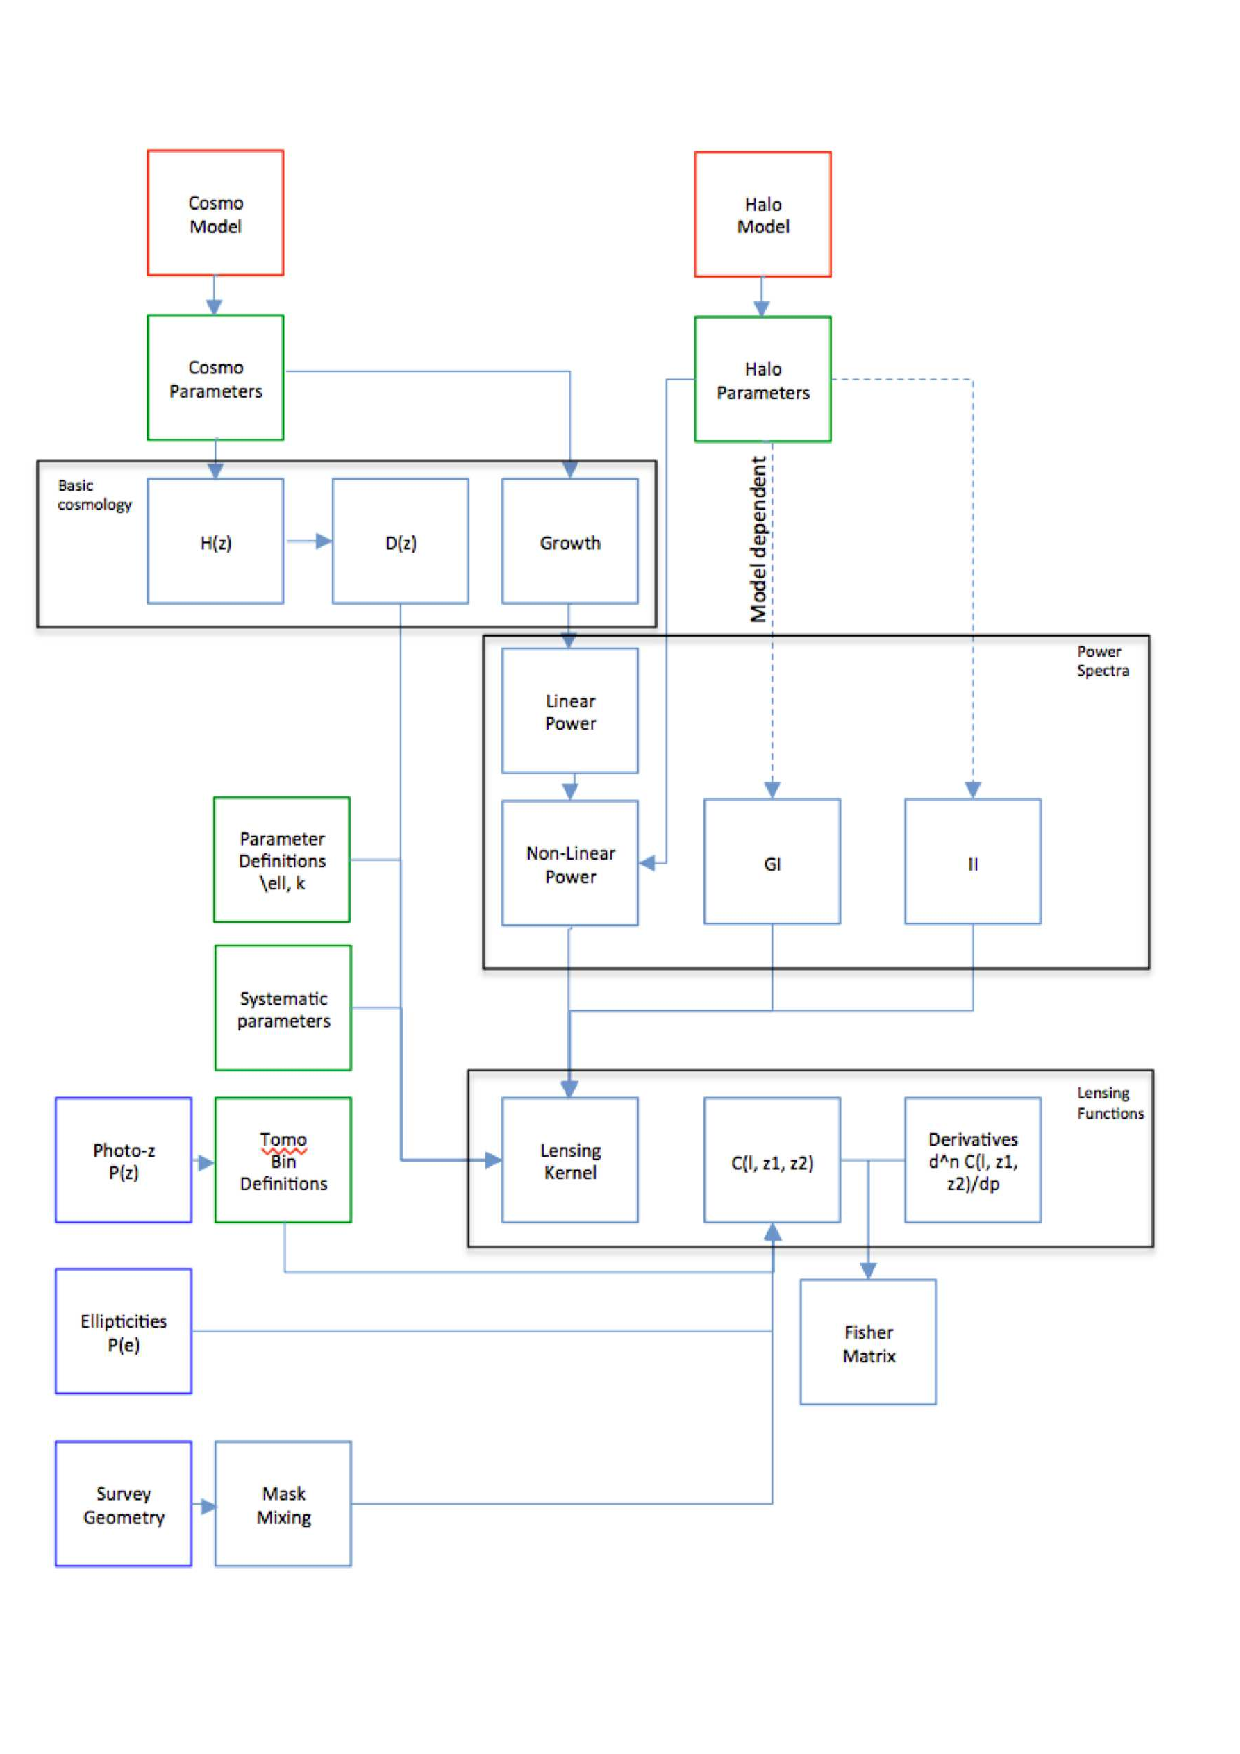
\includegraphics[angle=0,clip=,width=\columnwidth]{forecast_flow.pdf}
 \caption{Weak lensing tomographic theory-flow. {\bf discussion point: how detailed we make each box will be deligated to 
     individuals to take ownership over each PF. For example in the growth PF, this could/should rather be 
     for the whole Weyl potential $\Phi$ + $\Psi$.}}
 \label{WLtomo}
\end{figure}

\subsection{Galaxy Clustering: } 
TBW

\subsection{Weak Lensing+Galaxy Clustering: }
TBW 

\section{Coding, Requirements \& Verification} 
Here we discuss some aspects of the coding, requirements and verification of the PFs. 

\subsection{Requirements} 
Each processing function must have an associated requirement. A requirement 
must be necessary, unambiguous and tracable. These requirements will be of severable different types. For example 
\begin{itemize} 
\item 
Some processing functions will have trivial `existence' requirements flow that are simply to ensure that parameters 
exist in the specified header file and that they are read in correctly. These parameters will be expected to be traceable 
either to the Parameter definition document, GDPRD, OU RSD, or SciRD requirement in which the parameter is defined 
in exact detail; either a parameter of interest (i.e. cosmological) or a nuisance parameter (i.e. a systematic). 
\item 
Some processing functions will have numerical `budget allocations' that have flow-down from higher level breakdowns 
with regard to the top-level science objectives. For example an error on the Figure of Merit caused by binning in 
some quantity may have flow-down from a requirement that has shared a larger error-on-FoM budget with other 
PFs in the SGS or cosmological simulations PFs. 
\end{itemize} 

\subsection{Verification}
As well as requirements each PF will be expected to have a verification test associated with it. This means a specified 
set of tests that with known input produce known outputs such that the code can be verified to be computing what it 
is intended. In the case of theory-flows these verfication test should ideally be of a theoretical (analytic) nature 
in particular regimes of applicability, and numerical in others. 
Cross-validation verification tests are also encouraged for each PF, where several ($>2$) independently written 
codes can be compared and the output compared for each on. 

In the SGS as well as verification tests there are also `validation' tests that compare the PF outputs to calibration 
data. There is no such data in the theory-flow case, however there are retrodictive tests on current data that can be 
performed. These tests will require, where possible, the output of the functions and statistics to be tested against 
current data, which should be consistent with the outputs (albiet at much large tolerance than will be 
required for Euclid). Some PF may be more amenable for this, for example certain parts of PFs that involve 
CMB cross-correlations can be compared against Planck data. 

\subsection{Coding Standards}
We will adopt the same general coding practices as the SGS, in terms of language, library use and tracability. These
can be found in the SGS SIRD document. However, as it is expected to be scientists and not software engineers that 
create these codes, we do not adopt the next level of engineering i.e. the use of LODEEN and CODEEN environments. 

In order to facilitate code production we will use the following tools: {\bf to be dicussed, TBW} 

There is also the possibility of using external codes, outside Euclid for forecasting purposes. If this is the 
case a special committee will be formed and asked to assess the pros and cons of the use of such code, and the 
amount of time estimated to code a similar Euclid-specific version estimated. In the event that it is voted by the IST 
to be the best course to adopt such a code then the IST coordinators will form an  
MOU between the code authors and the Euclid IST should be sought, that should be done independently, and in 
addition to, the license agreements of the code. The MOU will cover in particular the ownership and license of any 
Euclid-specific modules that may contain prioritary information, authorship rights incurred, and so forth.



%%%%%%%%%%%%%%%%%%%%%%%%%%%%%%%%%%%%%%
\section{Forecasting Procedures} 
In this section we outline the two mechanisms through which robust forecasting for Euclid will be achieved. 

\subsection{Holistic Approach -- Comparing Currently Existing Pipelines}
%methodolgy for comparing current codes on an end to end basis   
The first approach will be to use \emph{existing} forecasting codes that are already at a mature stage. In this case
the full end-to-end theory-flow is being tested in a single step by comparing, for a given set of well defined inputs, 
the final Fisher matrix output or similar. In this it is required that
\begin{enumerate} 
\item 
The inputs are well defined and common to all forecasting pipelines (e.g. parameter definitions) 
\item 
That the outputs are well defined (e.g two-derivative Fisher matrix elements)
\item 
The metrics that will be used for the comparison (e.g. the DETF Figure of Merit), and a measure of agreement 
in these metrics that must be achieved in order to confirm that the codes are consistent.
\end{enumerate} 
In this case it is not possible to objective verify that any given code is returning the true performance, 
but the inter-subjectivity of more than one code can be verified by having many code do the comparison. 
In the event that there is inconsistency in the code then in the first instance simple debugging is encouraged and 
in the second instance an atomistic approach should be adopted. 

The holistic approach will result in inter-subjectively verified, consistent, forecasts for Euclid, but will not 
constitute a production of a verified Euclid theory code. For this we will pursue the atomistic approach below. 

The IST will provide for each theory-flow a set of templates that can be used to test forecasting pipeline in 
this holistic manner. These are provide in Appendices {\bf to be defined}. 

\subsection{Atomistic Approach -- Building a Euclid Cosmology Pipeline}  
Although the holistic approach to forecasting can result in forecasts that are external self-consistent, we also 
wish to build a theory code that verified to be both internal and externally self consistent. To this end 
we will develop the atomistic approach to forecast building where each PF in the theory-flow is compared on a case-by-case
basis, such that the result is a likelihood code that -- by construction -- has some objectively verified forecasting 
capability built into it. This approach is significantly slower than a holistic approach, which we will pursue for 
more short term forecasting objectives. 

For each PF the IST will create a series of PF requirements that must be met in order for the PF to be agreed to be 
usable. Each PF can be developed in isolation, although this may cause mis-matches between lower-level PF and 
upper-level ones when internal PF are written. Therefore we will pursue a `top-down' construction i.e. from the 
inputs subsequently down through the theory-flow to the output level. 
For each PF the requirement and verification will define 
\begin{enumerate} 
\item 
Analytic examples where the output can be verified against a known truth i.e. systems tests of the PF. That must be
reproduced at machine-precision. 
\item 
A series of numerical convergence tests that the PF must be shown to reach stability in. In particular for 
derivative and integral approximations. 
\item 
A series of metrics against which more than one independently code can be compared. These metrics should cover 
the whole range of functional output expected to be applicable for Euclid e.g. comoving distance at all redshifts, 
not only comoving distance `figure of merit', and such metrics should agree at machine-precision. 
\end{enumerate} 
We will pursue the construction of several theory pipelines written in several different languages such that 
language-specific libraries and assumptions are more ready identified as development moves down through the pipeline. 
At each stage a record must be kept of the requirements and evidence of the PF being passed. 

\subsection{Definition of Cosmological \& Nuisance Parameters} 
%need to define both 
Here we define the common set of cosmological and nuisance parameters that will be used as a starting point for 
both approaches to forecasting. 
\\
{\bf need to refer to the theory parameter definition document here.}
\\
References for GC: \cite{2003ApJ...598..720S}. References for WL: \cite{2006ApJ...636...21M}
General references on Fisher and Euclid: \cite{Amendola2010a, Euclid_TWG}

In the event that a SWG generates a new set of parameters, e.g. in the case that a new theory or new observations lead to the 
requirements that additional parameters are included in a forecast, this will be proposed by the SWG in question in a technical note 
written to the IST. The IST managers will then enter discussion with the SWG in question on 
the implementation. Any additional parameter will 
be recorded in the mission data base, and parameter definition documents, and this document will be updated accordingly in the even that 
a parameter is decided to be included. 

\section{Management of the IST} 
The IST will be subdivided into several workpackages to reflect the tasks at hand. These workpackages will be decided between the 
IST managers and the IST team, and recorded in the SWG Work Package Description document. Workpackages will be reviewed in an 
organic process, i.e. created and reviewed on a case by case basis as the need arises, on approximately a 6-month to 1-year rotating 
timetable.  

\section{End Comments}
This document does the following:
\begin{enumerate} 
\item 
Defines the scope of the IST with regard to the SGS, and SWGs. 
\item 
Contains and defines the theory-flow for the primary cosmological probes. 
\item 
Defines the procedure through which the primary cosmological probes forecasts will be constructed both through a 
holistic (end-to-end) approach and an atomistic (pipeline-building approach). 
\item 
In the following appendices describes the defined holistic procedure of the GC and WL primary probes. 
\end{enumerate}
The following will be captured in specific separate documents that will refer to this one. 
\begin{enumerate} 
\item 
Requirements and verification specifications for each of the primary cosmological probe theory-flows (one for each 
flow). 
\item 
Specifications of the atomistic specifications for each theory flow. 
\item
Results of the holistic and atomistic forecasts, these will appear documented as a Euclid technical notes, 
and may also lead to publications.  
\end{enumerate} 
The above documents will be recorded on the Euclid redmine and uploaded to the Euclid ESA RSSD under the SWG section 
when ratified.

\newpage

\section*{Appendix: Galaxy Clustering Holistic Forecast Definitions}\footnote{For the moment this part has been extracted from the TWG documentation of the code comparison, whose contributors were: L.Amendola, S. Camera, Santiago Casas, Enea Di Dio, Bin Hu, Elisabetta Majerotto, Valeria Pettorino, Domenico Sapone.}
We recall the main equations to be used. Observed linear spectrum at all redshifts:
\begin{equation} \label{eq:observed-power}
P_{r,obs}(k_{ref},\mu_{ref};z)=P_{s}(z)+\frac{D_{A}(z)_{ref}^{2} H(z)}{D_A(z)^{2} H_{ref}(z)} \frac{P(k,z)}{P(k,z=0)} b^{2}(z) (1+\beta(z)\mu^{2})^{2}P(k,z=0)\,,
\end{equation}
We use:
\begin{itemize}
\item For the linear matter power spectrum $P(k,z)$ $\rightarrow$ input files provided by Enea Di Dio and Bin Hu. 
\item For the growth index $f(z,k)$ (needed for $\beta_{d}(z)=f(z)/b(z)$), $\rightarrow$ input files provided by Enea Di Dio and Bin Hu (\revtext{k dependence not necessary. k fixed to k  = 0.1 h/Mpc). Input files need to be done differently for future tests}). 
\item For the $H(z)$ and $D_A(z)$ we use analytical expressions (see below, sec. \ref{sec:hd}). \revtext{SC checked that the analytical derivatives wrt $\omega_b$ and $\omega_c$ (calculated considering $h$ as a parameter) now match also the numerical ones.}
\end{itemize}

Here $b(z)$ is the bias (provided by column 5 of Tab.(\ref{tableGC})), $\beta(z)$
is the redshift-distortion factor, $P(k)$ is the undistorted
linear matter spectrum (provided in the input with the correct normalization), $\mu$ is the
direction cosine, $D_A$ is the angular diameter distance (provided in the input)
and H is the Hubble rate at the shell redshift $z$ (provided in the input). 
$P_{s}(z)$  is the $z$- dependent shot-noise correction due to discreteness in the survey. 
The subscript $ref$ (for `reference') indicates
quantities calculated in the fiducial model. In linear theory we have
$\beta_{d}(z)=f(z)/b(z)$ where $f(z) \equiv d\log G/d\log a$ is the growth
rate (f is provided directly in the input for every cosmology, G is the growth factor but you should not need it, the input provides directly the growth rate f).

The Fisher matrix for every redshift bin shell is integrated in k (\revtext{Right now doing the $\mu$ integral from 0 to 1 and multiplying the integrand by 2)}):
\begin{equation}
%F_{ij}=\frac{1}{8\pi^{2}}\int_{-1}^{+1}\dd\mu\int_{k_{min}}^{k_{max}}k^{2}\dd k\,\frac{\partial\ln P_{obs}(k,\mu)}{\partial\theta_{i}}\frac{\partial\ln P_{obs}(k,\mu)}{\partial\theta_{j}}\left[\frac{n(z)P_{obs}(k,\mu)}{n(z)P_{obs}(k,\mu)+1}\right]^{2}V_{s}\,.
F_{ij}=\frac{1}{8\pi^{2}}\int_{-1}^{1}{\rm d}\mu\int_{k_{\rm min}}^{k_{\rm max}} k^2\cdot {\rm d}k\frac{\partial\ln P_{obs}\left(z;k,\mu\right)}{\partial\theta_{i}}
\frac{\partial\ln P_{obs}\left(z;k,\mu\right)}{\partial\theta_{j}}\cdot \left[\frac{ n\,
P_{obs}\left(z; k,\mu\right)}{n\,P_{obs}\left(z; k,\mu\right)+1}\right]^{2}V_{\rm s}
\label{eq:pkfm}
\end{equation}
 \revtext{where the $\theta$'s are the parameters:  $\theta = \{\omega_c \equiv \Omega_{c_0}h^2,\omega_b \equiv \Omega_{b_0}h^2,h, n_s, \ln(10^{10}A_s), b_i, P_{s}\}$ ($\tau$ has been fixed to fiducial because it is degenerate when using only WL and GC).}

The input provides the spectra $P(z,k)$ (already corresponding to the $A_s$ normalization) and all other functions $f(z)$, $D_A(z)$, $H(z)$ for each model.

$n(z)$ is the galaxy number density at redshift $z$ and $V_{s}$
is the survey volume of the entire (so all $4 \pi$) redshift shell dz. The power spectra are all obtained numerically
by solving the background and perturbation equations of the system
for each value of the parameters and they are provided as input.


The derivative of the galaxy power spectrum, at each redshift (so $z$ is fixed in the middle of the bin), with respect to the parameters (in this case $\omega_c$) is:
\begin{align} 
\left.\frac{\mbox{d}\ln P_{{\rm obs}}\left(\bar{z},k,\mu;\theta_{i}\right)}{\mbox{d}\theta_{i}}\right|_{fid} & =\frac{\partial\ln P_{obs}\left(\bar{z},k,\mu;\theta_{i}\right)}{\partial\ln P_{s}(\bar{z})}\frac{\partial\ln P_{s}(\bar{z})}{\partial\theta_{i}}+\frac{\partial\ln P_{obs}\left(\bar{z},k,\mu;\theta_{i}\right)}{\partial\ln f(\bar{z})}\frac{\partial\ln f(\bar{z})}{\partial\theta_{i}}\nonumber \\
 & +\frac{\partial\ln P_{obs}\left(\bar{z},k,\mu;\theta_{i}\right)}{\partial\ln H(\bar{z})}\frac{\partial\ln H(\bar{z})}{\partial\theta_{i}}+\frac{\partial\ln P_{obs}\left(\bar{z},k,\mu;\theta_{i}\right)}{\partial\ln D_{A}(\bar{z})}\frac{\partial\ln D_{A}(\bar{z})}{\partial\theta_{i}}\nonumber \\
 & +\frac{\partial\ln P_{obs}\left(\bar{z},k,\mu;\theta_{i}\right)}{\partial\ln P(k,\bar{z})}\frac{\partial\ln P(k,\bar{z})}{\partial\theta_{i}}+\frac{\partial\ln P_{obs}\left(\bar{z},k,\mu;\theta_{i}\right)}{\partial\ln b(\bar{z})}\frac{\partial\ln b(\bar{z})}{\partial\theta_{i}}\label{eq:derivatives-of-lnPobs}\\
 & +{\color{red}\frac{\partial\ln P_{obs}\left(\bar{z},k,\mu;\theta_{i}\right)}{\partial k}\frac{\partial k}{\partial\theta_{i}}+\frac{\partial\ln P_{obs}\left(\bar{z},k,\mu;\theta_{i}\right)}{\partial\mu}\frac{\partial\mu}{\partial\theta_{i}}}\nonumber 
\end{align}

In general, one needs to include a redshift error $\sigma_z$ and further multiply:
$P_{obs} = P_{obs} e^{-k^2 \mu^2 \sigma_z^2/H(z)^2}$.
The last two terms are non-vanishing
if one takes the Alcock-Paczynski effect into account for $k$ and
$\mu$, since they are also affected by geometrical terms.

The derivatives
are:

\begin{subequations}
\begin{align}
\frac{\partial\ln P_{obs}\left(\bar{z},k,\mu;\theta_{i}\right)}{\partial\ln P_{s}(\bar{z})} & =\frac{1}{P_{obs}\left(\bar{z},k,\mu;\theta_{i}\right)} \label{der:pshot}\\
\frac{\partial\ln P_{obs}\left(\bar{z},k,\mu;\theta_{i}\right)}{\partial\ln f(\bar{z})} & =\frac{2\beta(\bar{z})\mu^{2}}{1+\beta(\bar{z})\mu^{2}}\\
\frac{\partial\ln P_{obs}\left(\bar{z},k,\mu;\theta_{i}\right)}{\partial\ln b(\bar{z})} & =\frac{2}{1+\beta(\bar{z})\mu^{2}} \label{der:bias}\\
\frac{\partial\ln P_{obs}\left(\bar{z},k,\mu;\theta_{i}\right)}{\partial\ln P(k,\bar{z})} & =1 \\
\frac{\partial\ln P_{obs}\left(\bar{z},k,\mu;\theta_{i}\right)}{\partial\ln H(\bar{z})} & =1 + \color{red} \frac{4\beta(z)\mu}{1+\beta(z)\mu^{2}}(-\mu(\mu^{2}-1))+\frac{\partial\ln P\left(\bar{z},k;\theta_{i}\right)}{\partial k}k\mu^{2} \\
\frac{\partial\ln P_{obs}\left(\bar{z},k,\mu;\theta_{i}\right)}{\partial\ln D_{A}(\bar{z})} & =  -2 + \color{red}\frac{4\beta(z)\mu}{1+\beta(z)\mu^{2}}(-\mu(\mu^{2}-1))+\frac{\partial\ln P\left(\bar{z},k;\theta_{i}\right)}{\partial k}k(\mu^{2}-1)
\end{align}
\label{eq: partial-derivs-subeqns}
\end{subequations}
{
All these terms are set as follows:
\begin{itemize}
\item $\frac{{\rm d}\ln P(\bar{z}, k)}{{\rm d}\theta_i}$ are numerical derivatives, coming from the input files (of course $P(\bar{z},k)$ does not depend on bias or $P_{s}$). \revtext{The input files are however provided at different k's; therefore, when calculating the derivative you need to interpolate in k first and then calculate the difference at fiducial ($1 \pm \epsilon$)}.
\item $f(\bar{z},k)$ is given by the input file: while in the input f is a function of k, for the comparison, we fix k = 0.1 h/Mpc. 
\item $\frac{{\rm d}\ln f(\bar{z})}{{\rm d}\theta_i}$ are numerical derivatives, coming from the input files (k fixed as above).
\item $\frac{{\rm d}\ln H(\bar{z})}{{\rm d}\theta_i}$ and $\frac{{\rm d}\ln D_A(\bar{z})}{{\rm d}\theta_i}$ are given by the analytical expressions described below (sec. \ref{sec:hd})
%\item $\frac{{\rm d}k}{{\rm d}\ln H(\bar{z})}$ and $\frac{{\rm d}\mu}{{\rm d}\ln H(\bar{z})}$ \revtext{for now are set to zero}.
%\item $\frac{{\rm d}k}{{\rm d}\ln D_A(\bar{z})}$ and $\frac{{\rm d}\mu}{{\rm d}\ln D_A(\bar{z})}$ \revtext{for now are set to zero}.
\end{itemize}
}
We tested three different methods: 
\begin{itemize}
\item Direct derivative: you integrate directly all terms of equation \ref{eq:derivatives-of-lnPobs} into eq.\ref{eq:pkfm};
\item Numerical derivative: evaluate the numerical derivative of eq.\ref{eq:pkfm} just calculating $P_{obs}(\bar{z},k)$ at $\theta_{i, fid} (1\pm \epsilon)$ and then divide by $2\epsilon \theta_{i, fid}$;
\item Jacobian method (or extended BAO Seo-Eisenstein method, see \cite{2003ApJ...598..720S}) 
\end{itemize}
All three methods match when there is no AP effect. With AP effect, the Jacobian method differs from the other two. For the following comparison, fisher matrices are provided using the direct derivative method.

\subsubsection*{The Hubble parameter and the angular diameter distance}\label{sec:hd}
We here assume that we consider h as a parameter, rather than $\Omega_{\Lambda}$.
The Hubble Parameter, for the cosmology we are using, is 
\be
H(z) = 100 h \sqrt{ \frac{\Omega_c h^2 + \Omega_b h^2+ \Omega_\nu h^2}{h^2} (1+z)^3 + 1 - \frac{\Omega_c h^2 + \Omega_b h^2+ \Omega_\nu h^2}{h^2}} \equiv 100 E(z) \,\,\, \textrm{[h km/s/Mpc]}
\ee
We then take into account the variation of $\omega_c = \Omega_{c,0}h^2$ and $\omega_b = \Omega_{b,0}h^2$.
The derivatives of the logarithm of Hubble parameter with respect to $\omega_c$, $\omega_b$ and $h$ are: 
\bea
\frac{\partial \ln H}{\partial \omega_c}{|}_{\omega_b, h} &=& \frac{(1+z)^3 -1}{2 h^2 E^2(z) }\\
\frac{\partial \ln H}{\partial \omega_b}{|}_{\omega_c, h} &=& \frac{(1+z)^3 -1}{2 h^2 E^2(z) }\\
\frac{\partial \ln H}{\partial h}{|}_{\omega_b, \omega_c} &=& \frac{1}{h E^2(z)} -\frac{1}{h}
\eea
and the other derivatives of the Hubble parameters with respect to $n_s$, $A_s$ and $\tau$ are clearly zero. Note that had we chosen $\Omega_i$ as variables instead of $\omega_i$, the derivative of the Hubble function with respect to h in units of [h km/s/Mpc] would have been zero.
The angular diameter distance is 
\be
D_A(z) = \frac{1}{H_0} \frac{c}{1+z} \int_0^z \frac{dx}{E(x)}
\ee
where $c$ is the speed of light and it is important to have distances in Mpc/h and 
\be
H_0 = \frac{100\,h\,{\rm Km/s/Mpc}}{c}= \frac{1}{2997.92}\frac{h}{{\rm Mpc}}\,.
\ee
The derivatives of the angular diameter distance are:
\bea
\frac{\partial \ln D_A}{\partial \omega_c} &=&  \frac{1}{D_A(z)} \frac{c}{1+z} \int_0^z - \frac{\partial \ln H(x)}{\partial \omega_c} \frac{dx}{H(x)}\\
\frac{\partial \ln D_A}{\partial \omega_b} &=&  \frac{1}{D_A(z)} \frac{c}{1+z} \int_0^z - \frac{\partial \ln H(x)}{\partial \omega_b} \frac{dx}{H(x)}\\
\frac{\partial \ln D_A}{\partial h} 		     &=&  \frac{1}{D_A(z)} \frac{c}{1+z} \int_0^z - \frac{\partial \ln H(x)}{\partial h} \frac{dx}{H(x)}
\label{eq:dlndadx}
\eea
All these derivatives will be used in the Fisher matrix. Galaxy density: take column 4 of Table (\ref{tableGC}), (dn3) as dn/dz/$d\Omega$ (with $\Omega$ in square degrees). There is no need to add in an
extra redshift success rate (e.g. epsilon=0.35) as before - this is already included in the numbers,
which now account for redshift- and flux-dependent success rate, in addition to using an improved
mock catalogues and redshift-measurement technique. There is also no need to include any scaling.
These numbers are for the standard integration time (540 sec per dither, standard dither pattern). As an
example, to get the total number of galaxies in a bin of width $0.95<z<1.05$, one would calculate:

(Number of galaxies $0.95<z<1.05$) = $4825.80 * 0.1 * 15000 = 7,239,000$

So in a Euclid survey over $15,000deg^2$ we would get good redshifts for $7,239,000$ galaxies in the
redshift range $0.95<z<1.05$. Note the 0.1 factor required to turn dn/dz from a derivative to a number in
a bin of width $Dz=0.1$.

This gives you the total number of galaxies. Then the number density that you need in the fisher for GC, $n$ in eq.\ref{eq:pkfm} in the formula for the fisher matrix, is the density per volume in each bin, therefore equal to: 
\begin{equation}
n = dn3 / dV_{dz} * dz 
\end{equation}
where the dz is the width of the redshift shell (i.e 0.1 but see the file) and 
\begin{equation}
dV_{dz} = \frac{\frac{4 \pi}{3} \left[ (1+z_2)^3 D_A[z_2;\theta]^3 - (1+z_1)^3 D_A[z_1;\theta]^3  \right]}{4 \pi \left(\frac{180}{\pi}\right)^2}
\end{equation}
is the volume in the redshift shell per degree squared.
The survey Volume is 
\begin{equation}
V_s = \text{Area} (\text{i.e. } 15,000 \text{ sq deg}) * dV_{dz}
\end{equation}

\revtext{The third column (dVol) should not be used anywhere.}

\begin{table}[htdp]
\caption{Specifications of the redbook, (derived from Orsi et al. 2009).}
\begin{center}
\begin{tabular}{c|c|c|c|c}
\hline
 {\bf zmin} & {\bf zmax} & {\bf dVol} & {\bf dn3} & {\bf b3} \\
\hline 
\hline
0.35 & 0.45 & 3.60 & 0.000 & 0.992 \\
0.45 & 0.55 & 5.10 & 0.000 & 1.024 \\
0.55 & 0.65 & 6.40 & 0.000 & 1.053 \\
0.65 & 0.75 & 7.90 & 2434.280 & 1.083 \\
0.75 & 0.85 & 9.20 & 4364.812 & 1.125 \\
0.85 & 0.95 & 10.30 & 4728.559 & 1.104 \\
 0.95 & 1.05 & 11.70 & 4825.798 & 1.126 \\
1.05 & 1.15 & 12.30 & 4728.797 & 1.208 \\
1.15 & 1.25 & 13.30 & 4507.625 & 1.243 \\
1.25 & 1.35 & 14.00 & 4269.851 & 1.282 \\
1.35 & 1.45 & 14.60 & 3720.657 & 1.292 \\
1.45 & 1.55 & 15.10 & 3104.309 & 1.363 \\
1.55 & 1.65 & 15.60 & 2308.975 & 1.497 \\
1.65 & 1.75 & 16.00 & 1541.831 & 1.486 \\
1.75 & 1.85 & 16.20 & 1474.707 & 1.491 \\
1.85 & 1.95 & 16.50 & 893.716 & 1.573 \\
1.95 & 2.05 & 16.70 & 497.613 & 1.568\\ 
\hline
\hline
\end{tabular}
\end{center}
\label{tableGC}
\end{table}%

\subsection*{GC comparison: where to start}
In Case 1,2,3 the following common options are fixed:
\begin{enumerate}
\item $k_{min}: 0.001$ h/Mpc
\item $k_{max} = 0.2$ h/Mpc
\item k-binning: use directly the one of the spectra provided in the input
\item No relativistic corrections.
\item Area : 15,000 sq deg
\item Redshift range : $0.7 < z < 2.0$
\item Binning: use all bins as in the table, starting from 0.65 (the first non-zero in dn3).
\end{enumerate}

\subsection*{GC case 1: minimal setting.}
In addition to the common settings above, use these settings for your first comparison.
\begin{enumerate}
\item  Bias: fixed to the fiducial value (column 5, b3 in the table \ref{tableGC}). All derivatives wrt the bias are zero.
\item The AP effect is zero: the four derivatives of k and $\mu$ with respect to H and $D_A$ are set to zero.
\item $P_{shot} = 0$ (fixed)
\item $\sigma_z = 0$
\end{enumerate}

\revtext{The Fisher matrix to compare with for this case, is case1.dat.}
If it matches, proceed to case2.

\subsection*{GC case 2: including the bias}
In addition to the common settings above, case2 fixes:
\begin{enumerate}
\item  Bias: marginalization over bias, derivatives as in \ref{der:bias}.
\item The AP effect is zero: the four derivatives of k and $\mu$ with respect to H and $D_A$ are set to zero.
\item $P_{shot} = 0$ (fixed)
\item $\sigma_z = 0$
\end{enumerate}

\revtext{The Fisher matrix to compare with for this case, is case2.dat.}

If it matches, proceed to case3.

\subsection*{GC case 3: including the AP effect}
In addition to the common settings above, case3 fixes:
\begin{enumerate}
\item  Bias: marginalization over bias, derivatives as in \ref{der:bias}.
\item The AP effect is included. 
\item $P_{shot} = 0$ (fixed)
\item $\sigma_z = 0$
\end{enumerate}

\revtext{The Fisher matrix to compare with for this case, is case3.dat.}

If it matches, proceed to case4.

\subsection*{GC case 4: including the shot noise}
In addition to the common settings above, case4 fixes:
\begin{enumerate}
\item  Bias: marginalization over bias, derivatives as in \ref{der:bias}.
\item The AP effect is included.
\item $P_{shot}$: marginalisation over $P_{shot}$; the fiducial is still zero; derivatives are calculated according to \ref{der:pshot} 
\item $\sigma_z = 0$
\end{enumerate}

\subsection*{GC case 5: Constraining  $ \,\ln D_A(z),\, \ln H(z),\,f\sigma_8(z), \, b\sigma_8(z),\, P_{s}(z) $ at each redshift bin}
In this case, we want to constrain some cosmological functions that depend on redshift, especially $f\sigma_8(z), \, b\sigma_8(z)$.


For doing this, we rewrite eqn. \ref{eq:observed-power} as: 
\begin{equation}
 P_s(z) + \frac{D_A(z)^2_\text{ref} H(z)}{D_A(z)^2 H_\text{ref}(z)}     \left(b\sigma_8(z) + f\sigma_8(z) \mu^2 \right)^2 \frac{P(k,z)}{\sigma^2_8(z)}
\end{equation}

The full list of parameters is the following:
\begin{itemize}
\item n cosmological parameters, in our case $n=5$: $\theta_i =\{ \Omega_c h^2,\, \Omega_b h^2,\, h,\, n_s,\, \ln 10^{10} A_s \}$
\item $5\times n_{bin}$ redshift-dependent parameters: $\{ \ln D_A(z),\, \ln H(z),\,f\sigma_8(z), \, b\sigma_8(z),\, P_{s}(z) \}$
\end{itemize}

Now we will have small modifications on the derivatives:

\begin{subequations}

\begin{align}
\frac{\partial\ln P_{obs}\left(\bar{z},k,\mu;\theta_{i}\right)}{\partial\ln P_{s}(\bar{z})} & =\frac{1}{P_{obs}\left(\bar{z},k,\mu;\theta_{i}\right)}\\
\frac{\partial\ln P_{obs}\left(\bar{z},k,\mu;\theta_{i}\right)}{\partial f \sigma_8(\bar{z},k)} & = \frac{2 \mu^2}{b\sigma_8(\bar{z}) + \mu^2 f \sigma_8(\bar{z},k)}\\
\frac{\partial\ln P_{obs}\left(\bar{z},k,\mu;\theta_{i}\right)}{\partial b\sigma_8(\bar{z})} & = \frac{2 }{b\sigma_8(\bar{z}) + \mu^2 f \sigma_8(\bar{z},k)}\\
\frac{\partial\ln P_{obs}\left(\bar{z},k,\mu;\theta_{i}\right)}{\partial\ln H(\bar{z})} & = 1 + \mu^2 \left(1 - \mu^2\right) \frac{ f \sigma_8(\bar{z},k)
  }{b\sigma_8(\bar{z}) + 
     \mu^2 f \sigma_8(\bar{z},k)} + k \mu^2 \frac{\partial \ln P(k,z)}{\partial k}\\
\frac{\partial\ln P_{obs}\left(\bar{z},k,\mu;\theta_{i}\right)}{\partial\ln D_{A}(\bar{z})} & =  
-2 + 4 \mu^2 \left(1 - \mu^2\right)\frac{ f \sigma_8(\bar{z},k)}{
  b\sigma_8(\bar{z}) + \mu^2 f \sigma_8(\bar{z},k)} - 
k (1 - \mu^2) \frac{\partial \ln P(k,z)}{\partial k}
\\
\frac{\partial\ln P_{obs}\left(\bar{z},k,\mu;\theta_{i}\right)}{\partial \theta_i} & = \frac{\partial \ln P(k,z)}{\partial \theta_i} - 
\frac{2}{\sigma_8(\bar{z})} \frac{\partial \sigma_8(\bar{z})}{\partial \theta_i}. \label{eq: partial-derivs-subeqns-sigma8}
\end{align}
\label{eq: partial-derivs-subeqns}

\end{subequations}

\revtext{The right hand side of eqn.\ref{eq: partial-derivs-subeqns-sigma8} is zero, when $\theta_i = \ln 10^{10} A_{s}$, so we should not add this parameter when constraining at the same time $\sigma_8(z)$.
A Fisher matrix for comparison, will be added once this detail is solved.
}

\section*{Appendix: Weak Lensing Holistic Forecast Definitions}

\subsection{Lensing projections}

Convergence power spectrum with (correlated) sources in redshift bins centered around $z_i$ and $z_j$ using Limber approximation:
\begin{equation}
P_{ij}(\ell)=\frac{9}{4}\int_{0}^{\infty}\mathrm{d}z\frac{W_{i}(z)W_{j}(z)H^{3}(z)\Omega_{m}^{2}(z)}{(1+z)^{4}}P_{m}\left(\frac{\ell}{ r(z)}\right),\label{eq:pstomog}
\end{equation}
 where $W_{i}(z)$ is the window function and r(z) is the comoving distance, which in flat space, is equal to the comoving angular diameter distance:
 \begin{equation}
r(z) = D_A(1+z)
 \end{equation}
This is provided in the input, column 3 of table VII. Please, for this comparison, do not use other methods to calculate it.
 
\begin{equation}
 W_i(z) = \int^\infty_z \frac{d\tilde{z}}{H(\tilde{z})}\left[ 1 - \frac{r(z)}{r(\tilde{z})} \right] n_i[r(\tilde{z})]
\end{equation}
where $r(z)$ is the coming distance.

\subsection{Redshift distribution}

The window function depends on $n_{i}(z)$, the galaxy distribution
in the $i$-th redshift bin: this is convolved with a Gaussian to account for photometric
redshift errors $\sigma_{z}$~(value specified below), i.e. 
\begin{equation}
n_{i}(z)=A \int\limits _{i\text{-th bin}}n({z})\exp\left(\frac{-(\tilde{z}-z)^{2}}{2 \sigma_{z}^{2}}\right)\mathrm{d}\tilde{z}
\label{n_binned}
\end{equation}
 where the integral is done over $\tilde{z}$ for the single i-th bin. 
$A = \frac{1}{\sqrt{2\pi} \sigma_z}$ a normalization factor.
In eq. (\ref{n_binned}), the density is given by: 
\begin{equation}
n(z) = z^2 exp(-(z/z_0)^{3/2})
\end{equation}
where $z_0 = z_{mean}/1.412$ is the peak of $n(z)$ and $z_{mean}$ is the median redshift (value specified below).

\subsection{Likelihood function}


\subsection{Covariance matrix}


\subsection{Real-space forecasts}


\subsection{Systematics}


\subsubsection{Instrumental and observational systematics}


\subsubsection{Astrophysical systematics}


\subsection{Intrinsic alignment}

\subsection{Non-linear power spectrum}


\subsubsection{Baryonic corrections}


\subsection{Fisher matrix}

Then the Fisher matrix is summed over all multiples:
\begin{equation}
F_{\alpha\beta}=f_{\mathrm{sky}}\sum\limits _{\ell,i,j,k,m}\frac{(2\ell+1)\Delta\ell}{2}\frac{\partial P_{ij}(\ell)}{\partial\theta_{\alpha}}C_{jk}^{-1}\frac{\partial P_{km}(\ell)}{\partial\theta_{\beta}}C_{mi}^{-1}\label{eq:fm-wl}
\end{equation}
 with the covariance matrix 
\begin{equation}
C_{jk}=P_{jk}+\delta_{jk}\gamma_{\mathrm{int}}^{2}{{{q}}_j}^{-1},
\end{equation}
 where $\gamma_{\mathrm{int}}$ is the
intrinsic galaxy shear  and 
\begin{equation}
q_{j} = 3600\left(\frac{180}{\pi}\right)^{2} n_{\theta} \int^\infty_0 n_j(z) dz \, .
\end{equation}
Here $n_{\theta}$ is the galaxy density per $\mathrm{arcmin}^{2}$ and $n_j(z)$ is the galaxy density for the j-th redshift bin, as defined in eq.(\ref{n_binned}).

Since we consider multipoles up to $\ell_{\mathrm{max}}=5000$,
we need to apply non-linear corrections to the matter power spectrum,
for which we use the halofit (provided in the input spectra).

\paragraph{Specifications for the weak lensing:}
\begin{enumerate}
\item Area: 15,000 sq deg
\item $f_{sky} = Area/(4 \pi (180/\pi)^2)$
\item Median Redshift: $z_{mean} = 0.9$
\item $\gamma_{\mathrm{int}}=0.22$
\item $n_\theta =$ 30 galaxies per $\mathrm{arcmin}^{2}$
\item Error on photometric redshift: $\sigma_z$ = 0.05 (1+z)
\item Linear Power Spectrum: CAMB (provided in the input, you shouldn't use it)
\item Method to correct for non-linearities: Halo model  (however the input files are now linear; it does not matter for now as we are not looking for the correct Fisher, just comparing. For this comparison we are using linear spectra).
\item Binning: 10 bins from z = 0 - 2.5. We assume equipopulated bins: the redshift bins chosen such that each contain
the same amount of galaxies. \comment{need to add formula}
\item k-range: $k_{min}=0.001$ h/Mpc, \revtext{$k_{max}=0.5$ h/Mpc}
\item k-binning: use directly the one provided in the input
\item $\ell$-range: $\ell_{min}=5$, $\ell_{max}$ \revtext{fixed as a function of z, using the table provided by Enea (uploaded in the wiki). No cut in z.}
\item $\ell$-binning: 100 bins (with log spaced binning)
\end{enumerate}

%\end{document}





\newpage
%\documentclass{Latex_Euclid_style}

%\usepackage{amsmath}
%\usepackage{amsfonts}
%\usepackage{amssymb}
%\usepackage{graphicx}
%\usepackage{epsfig}
%\usepackage[hang,small,bf]{caption}
%\usepackage{rotating}


% --------------

%\begin{document}

\section{Splinter Group 1: numerical codes}

\subsubsection*{Coordinators}
\begin{itemize}
 \item Valeria Pettorino, Matteo Martinelli
\end{itemize}
\subsubsection*{Participants}
\begin{itemize}
 \item Matteo Costanzi,  Yabebal Fantaye, Martin Kunz, Massimiliano Lattanzi, Julien Lesgourgues, Baojiu Li, Matteo Martinelli, Federico Marulli, Valeria Pettorino, Marco Raveri, Valentina Salvatelli, Barbara Sartoris, Luca Amendola, Thejs Brinckmann, Ziad Sakr
\end{itemize}

\subsubsection*{Aim}
Make a recommendation on existing codes for Atomistic Forecasting approach.\\
Expected output:
\begin{itemize}
 \item A technical note explaining pros and cons of the various potential public codes for this purpose 
 \item How do they meet our requirements:
 \begin{itemize}
  \item on the division/requirements setting at fine-grained level 
  \item on individual probe work and on combinations
 \end{itemize}
 \item Make a consensus of codes, and make a short presentation showing initial pros and cons.
\end{itemize}

\newpage
\subsection{Boltzmann codes}
This section includes an overview of publicly available Boltzmann codes. For each code we present a schema in the same format, including pros and cons.

\subsubsection{Requirements to trust a code in Modified Gravity}

For every MG model, there should be at least 2 Boltzmann codes, agreeing. Agreement is defined as follows: 
\begin{itemize}
 \item check them on LCDM, need to agree at less than 0.1\%
 \item check them in a MG scenario in different ranges of parameters: they should match at the same level at which they agree in LCDM on 
all background quantities, all perturbation quantities, all spectra
\end{itemize}

\newpage
\subsubsection{CAMB}
%\href{http://camb.info/}{CAMB}
(\url{http://camb.info/})\\

{\it \bf Language:} fortran90\\

{\it \bf Includes:}
\begin{itemize}
 \item standard neutrinos, sterile neutrinos
 \item CDM
 \item DE: $w_0\ w_a$
\end{itemize}

{\it \bf Pros: }
\begin{itemize}
%publicly available
 \item updated very often
 \item tested by a large community
 \item there are several implementations for MG models (though not as well tested)
 \item python wrapper for CAMB to join to any MCMC
 \item documentation available and often updated: quick feedback by Anony Lewis and large community, via cosmocoffee
\end{itemize}

{\it \bf Cons:}
\begin{itemize}
 \item structure of the code requires to modify different parts of the code for different models
 \item no general distribution function for neutrinos
 \item only synchronous gauge
 \item maintainer (Antony Lewis) not currently in Euclid
\end{itemize}

\newpage
\subsubsection{EFTCAMB}
(\url{http://wwwhome.lorentz.leidenuniv.nl/~hu/codes/})\\

{\it \bf Language:} fortran90\\

{\it \bf Includes:}\\

{\it \bf Pros:}
\begin{itemize}
 \item based on CAMB
 \item very general parametrization for effective field theory (EFT) parametrisation of MG and DE models
 \item tested against HiCLASS/MGCAMB/private codes for some models
 \item several parameterisations of the background expansion and also of the perturbations (now including the Horndeski functions)
 \item perturbation evolution computed self-consistently for EFT class of models
 \item Very clearly written, structured, documented. 
 \item It has a MCMC wrapper.
\end{itemize}

{\it \bf Cons: }
\begin{itemize}
 \item need further testing
 \item needs some understand stability conditions
 \item MG starts from z = 100 (not tested earlier)
\end{itemize}

\newpage
\subsubsection{MGCAMB}(\url{http://aliojjati.github.io/MGCAMB/})\\

{\it \bf Language:} fortran90\\

{\it \bf Includes: }
\begin{itemize}
 \item changes the response of the scalar metric potentials (phi and psi) to the perturbations: this can be due to modifications of the Einstein equations 
 (modified gravity) or due to extra clustering components (dark energy)
\end{itemize}

{\it \bf Pros: }
\begin{itemize}
 \item it works with some well tested parametrization; easy to compare with previous results 
 \item can test  very general deviations from LCDM visible in the scalar metric perturbations
\end{itemize}

{\it \bf Cons: }
\begin{itemize}
 \item When used as a ‘EFT replacement’:
 \begin{itemize}
  \item does not evolve all perturbation equations 
  \item assumes quasi static limit
 \end{itemize}
 \item General deviations in scalar metric perturbations require careful parameterisation, some further developments (eg. Gaussian process) may be required
 \item Does not include similar deviations in vector and tensor perturbations
 \item Works with $\Lambda$CDM background
\end{itemize}
Warning: the code was recently updated (late february). These comments do not refer to the latest version.\\

\newpage
\subsubsection{CLASS}(\url{http://class-code.net/})\\

{\it \bf  Language:} C

{\it \bf Includes:}
\begin{itemize}
 \item various forms of neutrinos and dark matter
 \item DE with a given equation of state, quintessence with scalar potentials.
 \item DE extension is HiClass but not public (Bellini, Miguel Zuma)
 \item newtonian and synchronous gauge
\end{itemize}

{\it \bf Pros: }
\begin{itemize}
 \item structure of code
 \item python wrapper
 \item two gauges (newtonian and synchronous: except the initial conditions which are only written in the synchronous gauge and gauge-transformed). 
 \item maintainer (Julien Lesgourgues) is active Euclid member
\end{itemize}

{\it \bf Cons: }
\begin{itemize}
 \item community that uses/tested CLASS is smaller than CAMB
\end{itemize}


\newpage
\subsection{Parameter estimation codes}
This subsection includes an overview of publicly available codes to calculate the likelihood.

\subsubsection{Requirements for parameter estimation codes}

The basic requirement for codes which obtain cosmological predictions from Boltzmann codes and perform parameter estimation is ``modularity''.\\
A modular code is easy to modify in case some changes and updates need to be included, e.g. additional likelihoods, extra parameters, correction to observables (systematics).\\
Furthermore, separate modules for different physical quantities are needed for the atomistic approach as they allow to easily retrieve and compute the intermediate quantities of the theory
flows (see e.g. Fig. \ref{WLtomo}) and to compare them between different codes.\\
However too much modularity may affect code performances.\\

A wishlist of modules is:
\begin{enumerate}
 \item module calling the Boltzmann/transfer function codes for primary science
 \item module calling the sampler
 \item module for each likelihood for each probe
 \item module for background quantities
 \item module for perturbation quantities
 \item module for non-linear corrections (ex. halofit)
 \item module that gets the standard output from Boltzmann codes and produces list of suitable output
 \item postprocessing of the samples
 \item plotting modules 
\end{enumerate}

In the following, the publicly available codes are listed, together with the requirements which are satisfied by each of them. The missed requirements are also listed and the complexity 
of implementation is indicated as easy (E), medium (M) and difficult (D)

\newpage
\subsubsection{COSMOMC}
(\url{http://cosmologist.info/cosmomc/})\\

{\it \bf Language:} fortran90\\

{\it \bf Pros:}
\begin{itemize}
 \item updated constantly
 \item very well tested, very efficient for standard cosmology
 \item used by a large community
 \item easy to add parameters
 \item easy to add an additional likelihood by adding a separate module
 \item nice python graphical interactive interface for first tests
 \item well documented
 \item there are many options and more control to analyse the samples. 
 \item Updated to all currently available data (WL, GC, clusters, CMB).
 \item Likelihood Sampler works really well
\end{itemize}

{\it \bf Cons: }
\begin{itemize}
 \item if you increase the number of parameters, the sampler gets slower. Other samplers are publicly available and already interfaced with COSMOMC. However they are not included in the 
 standard version (interface needs to be modified when COSMOMC is updated)
 \item maintainer (Antony Lewis) not currently in Euclid
\end{itemize}

{\it \bf Wish-list requirements: }
\begin{itemize}
 \item included: 1, 2 (add samplers), 3, 6, 8, 9
 \item missing: 4 (E CAMB has background functions collected in module ModelParams in modules.f90 which can be called by COSMOMC), 5 (D), 6 (alternatives to halofit), 7 (E/M) 
\end{itemize}

\newpage
\subsubsection{MONTEPYTHON}(\url{https://github.com/baudren/montepython_public} or \url{http://baudren.github.io/montepython.html})\\

{\it \bf Language:} python\\

{\it \bf Includes:}
\begin{itemize}
 \item Euclid mock likelihood (weak lensing + galaxies) is publicly available
 \item CMB, SNIa, BAO, WiggleZ (CHFTLens and SDSS to be released); 
\end{itemize}

{\it \bf Pros: }
\begin{itemize}
 \item modular environment
 \item can switch among different samplers
 \item it has a graphical interface
 \item can easily be interfaced with different Boltzmann codes
 \item can use MPI
 \item extra parameters need to be included only in the input file
 \item easy to add a new likelihood.
\end{itemize}

{\it \bf Cons:} 
\begin{itemize}
 \item community that uses/tested MP is smaller than COSMOMC
 \item less frequently updated 
\end{itemize}

{\it \bf Wish-list requirements: }
\begin{itemize}
 \item included: 1 (for generic Boltzmann code; currently points at Class wrapper; Camb wrapper in preparation), 2 (MH, Multinest, CosmoHammer, importance sampling, reprocessing chains, fisher matrices), 3, 4, 5, 6 (Halofit), 7, 8, 9 (can choose between MontePython or Getdist to produce plots or reprocess: chains are in the same format as cosmomc and can use 8,9 from COSMOMC) 
 \item missing: 6 (alternatives to Halofit E/M) 
\end{itemize}

\newpage
\subsubsection{COSMOSIS}(\url{https://bitbucket.org/joezuntz/cosmosis/wiki/Home})\\

{\it \bf Language:} ??\\

{\it \bf Includes: }
\begin{itemize}
 \item sampler code (http://arxiv.org/pdf/1409.3409v1.pdf)
 \item CFHTLens, Planck, some BAO, SNae JLA. 
\end{itemize}

{\it \bf Pros:} 
\begin{itemize}
 \item can be wrapped to CAMB and CLASS
 \item it is modular (can introduce other samplers or Boltzmann codes) 
 \item can add modules in different languages
 \item new parameters are defined only in the input parameter file
 \item They will include SDSS. Easy to implement a new module for a new likelihood.
 \item Used by DES.
\end{itemize}

{\it \bf Cons:} 
\begin{itemize}
 \item not very well tested
 \item small community uses it
 \item who is updating it?
\end{itemize}

{\it \bf Wish-list requirements: }
\begin{itemize}
 \item included: 1 (generic Boltzmann code: CAMB, CLASS), 2 (MH, MultiNest, EMCEE), 3 (...add…), 4 (?), 6 (Halofit, Halofit + T correction), 7
 \item Datablock the object passed down the pipeline. For a given set of parameters all module inputs are read from the datablock and all module outputs are written to it 
 \item missing: 4 (E but not implemented?), 5 (?), 6 (alternatives to Halofit; E/M), 8 (format of chains? can one use getdist? how advanced as compared to getdist?), 9 (how advanced with respect to COSMOMC ones?) 
\end{itemize}

\newpage
\subsubsection{NumCosmo}(\url{http://www.nongnu.org/numcosmo/})\\

\paragraph{emcee}(\url{http://dan.iel.fm/emcee/current/})\\
{\it Language:} python\\
{\it Includes:}
\begin{itemize}
 \item 3 different samplers (unified calling interface) and plotting tools
\end{itemize}
{\it Pros:} 
\begin{itemize}
 \item affine invariant sampling for fast sampling of degenerate likelihoods
 \item parallel tempered sampler for multimodal likelihoods
 \item standard Metropolis-Hastings sampler
 \item many plotting tools included
 \item can use MPI
 \item interfaces reasonbly easy to write
 \item interface to lensing code exists (in C)
 \item interface to supernova code exists (in C or python)
 \end{itemize}
{\it Cons:} 
\begin{itemize}
 \item not specifically interfaced to a Boltzmann code
\end{itemize}
{\it Wish-list requirements: }
\begin{itemize}
 \item inclusion of observables CMB, CMB-lensing, CMB cross-correlations (iSW) and galaxy clustering
 \item call to Boltzmann code (Bjoern: we’re working to add CMB-related probes)
\end{itemize}


\subsection{Code recommendation}

\paragraph{Coding Language}
The SGS use python and C++ only, and it would be good for us to follow them to have some coherence. Although there are pros and cons.\\
It would be ideal to have a python infrastructure: wrappers in python to other codes written in different open sources free languages (instead of IDL, Mathematica)\\
FR software to convert languages from one to another: help to write a python wrapper, for example SDC is using swig (http://www.swig.org/).
Good experience with SWIG, it serves as a way of passing data between python and other languages (Bjoern: tried out python$\rightarrow$C with openMP-parallelisation)\\
Make sure all libraries used/needed are available. 
SDC already has a list of libraries that are allowed to be used, at \url{http://euclid.roe.ac.uk/projects/codeen-users/wiki/EDEN}.
Python slow for high level performances, 

%\paragraph{Infrastructure}

\paragraph{Boltzmann code}

No specific choice, but recommendation is that we need at least 2 codes that match for each model (match in the sense explained above); 
in addition, our recommendation is to use MGCAMB only for tests (and clearly specify limitations of the code and assumptions in it)


\paragraph{Parameter estimation}
MontePython at present is the one that includes the highest number of requirements in the wish list. JL \& team within Euclid guarantee fast 
update for wrappers to Boltzmann code version updates and to new data which become available. 

\paragraph{Analysis and visualization}
Getdist and plotting tools provided by cosmomc

\paragraph{Code testing}
Self-consistent check of the likelihood codes:  use a simulation to produce a set of data and check if we can recover the initial cosmological model.\\
Available simulations: \\
galaxy mock catalogue
\begin{enumerate}
 \item from MICE simulations (HOD) in LCDM cosmology  \url{http://internal.euclid-ec.org/?page_id=1551}
 \item from Durham simulations (SAM) in LCDM cosmology 
\end{enumerate}
Needed:
\begin{itemize}
 \item simulations from non-standard cosmological models: e.g. f(R), DE 
 \item mock catalogue for WL (to be asked to the WL splinter-2
\end{itemize}


\paragraph{Required output from other groups}
\begin{itemize}
 \item SDC: list of python libraries (\url{http://euclid.roe.ac.uk/projects/codeen-users/wiki/EDEN})
 \item TWG:
 \begin{itemize}
  \item parameter definition document
  \item list of Boltzmann codes available for MG
 \end{itemize}
 \item Simulations: list of simulations available
\end{itemize}





%\end{document}





\newpage
% group2.tex

\section{Splinter Group 2: Weak Lensing Holistic Forecast Definitions}

\subsection{Lensing projections}

\mk{Generalized equations for non-flat Universe.}

The simplest form of the convergence power spectrum with (correlated) sources in redshift bins centered around $z_i$ and $z_j$ is
%
\begin{equation}
P_{ij}(\ell) = \frac{9}{4} \Omega_{\rm m}^2 \left(\frac{H_0}{c}\right)^3 \int_{0}^{z_{\rm lim}}\mathrm{d}z\frac{(1+z)^2}{E(z)} W_{i}(z)W_{j}(z)
    P_{\rm m}\left(\frac{\ell}{ f_K[r(z)], z}\right),
  \label{eq:pstomog}
\end{equation}
%
where $W_{i}(z)$ is the window function, $r(z)$ is the comoving distance, and $f_K$ the comoving angular
diameter distance as a function of curvature $K$. The function $E$ is related to the Hubble parameter as
%
\begin{equation}
  E(z) = \frac{H(z)}{H_0}.
  \label{eq:E}
\end{equation}
%
This
approximate expression uses the Limber approximation (collecting only modes
that lie in the plane of the sky, thereby neglecting correlations along the
line of sight, \cite{1953ApJ...117..134L,1992ApJ...388..272K}), the small-angle
approximation (expanding to first order trigonometric functions of the angle)
and the flat-sky limit (replacing spherical harmonics by Fourier transforms).
See Sect.~\ref{sec:WL_systematics} for further discussions on these astrophysical systematics.
The function $r$ is the comoving distance, which is related to the angular diameter distrance $D_{\rm A}$ as
%
\begin{equation}
  r(z) = D_{\rm A}(z) (1+z)
\end{equation}
%
 
\begin{equation}
 W_i(z) = \int^{z_{\rm lim}}_z {\rm d}\tilde{z} \, \frac{f_K[r(z) - r(\tilde z)]}{f_K[r(\tilde{z})]} n_i(\tilde{z})
\end{equation}
where $r(z)$ is the coming distance. The redshift distribution for bin $i$ is denoted with $n_i$, and it is normalized to
the number of galaxies belonging to that bin,
%
\begin{equation}
  \int_0^{z_{\rm lim}} {\rm d} z \, n_i(z) = 1.
\end{equation}
%
\mk{Modified, $n$ should depend on $\bar z$, not on $r$}

\subsection{Redshift distribution}

The window function depends on $n_{i}(z)$, the galaxy distribution
in the $i$-th redshift bin: this is convolved with a Gaussian to account for photometric
redshift errors $\sigma_{z}$~(value specified below), i.e.~
\begin{equation}
n_{i}(z)=A \int\limits _{i\text{-th bin}}n({\tilde z})\exp\left(\frac{-(\tilde{z}-z)^{2}}{2 \sigma_{z}^{2}}\right)\mathrm{d}\tilde{z}
\label{n_binned}
\end{equation}
 where the integral is done over $\tilde{z}$ for the single i-th bin. 
$A = \frac{1}{\sqrt{2\pi} \sigma_z}$ a normalization factor.
In eq. (\ref{n_binned}), the density is given by: 
\begin{equation}
n(z) = z^2 exp(-(z/z_0)^{3/2})
\end{equation}
where $z_0 = z_{mean}/1.412$ is the peak of $n(z)$ and $z_{mean}$ is the median redshift (value specified below).

\subsection{Likelihood function}


\subsection{Covariance matrix}


\subsection{Real-space forecasts}

The numerical calculation of real-space quantities is straight-forward,
accurate, and fast. All real-space functions can be represented as  1D
integrals over the filtered convergence-power spectrum $P_\kappa = P_\kappa^{\rm E} + P_\kappa^{\rm B}$.
For the 2PCF $\xi_+$
and $\xi_-$, these are efficiently carried out as Hankel transformation,
%
\begin{align}
  \xi_+(\theta) & = \frac 1 {2\pi} \int {\rm d} \ell \, \ell {\rm J}_0(\ell
   \theta)
  [ P_\kappa^{\rm E}(\ell) + P_\kappa^{\rm B}(\ell)];
  \nonumber \\
   %
   \xi_-(\theta) & = \frac 1 {2\pi} \int
   {\rm d} \ell \, \ell {\rm J}_4(\ell \theta)
  [ P_\kappa^{\rm E}(\ell) - P_\kappa^{\rm B}(\ell) ].
  %
   \label{eq:xi_pm_pkappa}
\end{align}
%
For COSEBIs, the aperture-mass dispersion, and other real-space functions, the
filter functions are smooth and have none to relatively few oscillations.
The general expression for an E-/B-mode separating function $X_{\rm E, B}$ is
%
\begin{equation}
  X_{\rm E, B} = \frac 1 {2\pi} \int_0^\infty {\rm d} \ell \, \ell \, P_\kappa^{\rm E, B}(\ell) \fourier U^2(\ell) .
  %
  \label{eq:X_EB_Fourier}
\end{equation}
%
Fast
and acurate codes exist to carry out the integrals in (\ref{eq:xi_pm_pkappa}) and (\ref{eq:X_EB_Fourier})
(\texttt{FFTLog} \cite{2000MNRAS.312..257H};
\texttt{nicaea}, part of \texttt{CosmoPMC} \cite{cosmo_pmc_ascl}; non-public
codes from Patrick Simon, Marika Asgari).

Some of these transformations are valid for a flat sky, and we need to check
their accuracy for the curved sky case, and potentially modify those
tranformations if necessary.

The covariance matrix for real-space functions often shows stronger
off-diagonal parts than the power spectrum. The latter, in the ideal case of a
Gaussian shear field on the full sky, has zero-off diagonal elements. However,
the non-Gaussian LSS on small scales and mask effects introduce off-diagonal
correlations. In fact, the relation between the observable (band-power)
spectrum and the underlying true convergence power spectrum $P_\kappa$ has the
same form (\ref{eq:X_EB_Fourier}) as the relation between a real-space function
and $P_\kappa$. The amplitude of off-diagonal elements depends mainly on the
width of the filter function.

$\xi_+$ and $\xi_-$ have a covariance with very large off-diagonal elements.
The calculation of the cosmic variance term even in the Gaussian case is
time-consuming due to the product of two Bessel function with different
arguments $\ell \theta_i$, $\ell \theta_j$ for the off-diagonal element
$C_{ij}$ with $i \ne j$. Code exists (Benjamin Joachimi) that has been used
within Euclid. Even with parallelization on ${\cal O}(50)$ CPUs, 
for $N_\theta = 50$ and $N_z = 12$ it takes a up to two weeks to compute
the $N_\theta^2 [N_z (N_z + 1)] / 2 \times 4$ covariance elements for $\xi_+$ and $\xi_-$
including the mixed terms ($+-, -+)$.



\subsection{Systematics: overview}
\label{sec:WL_systematics}

Often for Fisher matrix forecast, we implicitly assume that the observed power spectra
is an unbiased realization of the underlying theoretical one so that we can
directly compare them to infer constraints on the cosmological parameters.
Actually, systematics make this assumption less than obvious. Roughly speaking,
we can divide systematics sources in three classes.

\begin{itemize}

\item{\it Astrophysical/theoretical systematics.} This includes all those
lensing-related effects which are usually taken for granted and neglected in the standard
analysis. These are listed in Sect.~\ref{sec:lensing_systematics}, with the exception
of intrinsic aligment (IA). As one of the dominant contaminations of the lensing signal,
IA is discussed in the separated Section \ref{sec:IA}.

\item{{\it Instrumental systematics.} Textbook example is CTI correction which
introduces an artificial distortion pattern which impacts the ellipticity of
each galaxy and hence the shear determination. As a result, a fake correlation
can be induced leading to a biased observed power spectrum.} \\

\item{{\it Observational systematics.} These are related to errors in the
measurement process. The most well known case concerns shape measurement codes.
In a first good approximation, one can assume that the measured ellipticity
$\epsilon_{obs}$ is related to the true one $\epsilon$ as $\epsilon_{obs} = (1
+ m) \epsilon + c$, with $(m, c)$ the multiplicative and additive bias
respectively. Depending on the code, $(m, c)$ can depend on the galaxy
properties; e.g.~\cite{CFHTLenS-shapes} have used mock CFHTLenS data analysed
with the {\it lensfit} code to show that, while $c$ is negligible, $m$ is a
function of the galaxy size and S/N ratio. As a second example, one can
consider colour gradient bias which can still be parameterized with the same
formalism with $m$ dependent on the source redshift and color as preliminarily
found by \cite{2013MNRAS.432.2385S}.}

\end{itemize}

The impact of systematics in the first class can be explicitely evaluated and their impact on the cosmic shear power spectrum quantified and included if necessary. On the contrary, second and third class systematics ask for a more empirical analysis. Under general assumptions, we can model their impact stating that the following relation hold

\begin{displaymath}
{\cal{C}}_{sys}(\ell, z_i, z_j) = (1 + {\cal{M}}_{ij}) {\cal{C}}_{lens}(\ell, z_i, z_j) + {\cal{A}}(\ell, z_i, z_j)
\end{displaymath}
where ${\cal{C}}_{sys}$ and ${\cal{C}}_{lens}$ are the cosmic shear power spectra with systematics included and the theoretical one, ${\cal{M}}_{ij}$ a redshift dependent multiplicative correction and ${\cal{A}}(\ell, z_i, z_j)$ is a scale and redshift dependent additive correction.

Forecasting codes should include the relevant astrophysical systematics as a first step. A parameterization for the multiplicative and additive bias terms should be worked out to be added as soon as second and third class systematics have been quantified in some way.




% -------------------------------------------------------------------- %
\subsection{Systematics: astrophysical}
\label{sec:lensing_systematics}

Weak lensing probes the cosmic large-scale structure through its null-geodesics: While this property follows almost universally from all relativistic theories of gravity and is easy enough to understand, the technical computation of weak lensing observables, in particular on small scales, is challenging as it is influenced by a number of second-order effects. With Euclid, large multipoles are probed with high statistical precision such that the exact prediction of spectra on small scales is necessary in order to have unbiased measurements: Euclid's weak lensing data set will have a statistical significance of about $10^3\sigma$, such that for example an over- or underpredicition of the spectra by $10^{-3}$ will be a $1\sigma$-bias.

Second order effects in weak lensing fall into a couple of categories, according to the physical mechanisms, but they have in common that the weak lensing signal is weighted by a second field, which, under some circumstances, can generate $B$-modes in the ellipticity field - with impact on the calibration of the ellipticity measurements. Typically, the effects are important on small scales around and above $\ell=10^3$ and modify the spectra by a factor of $10^{-3\ldots-8}$ depending on the nature of the weighting field.

\subsubsection{geodesic effects}
The implict lens equation is solved by a perturbative expansion, where the weak lensing deflection is collected by integration along a straight line replacing the actual light path. At higher order, there are corrections due to better approximations of the actual light path (Born-corrections). Similarly, the change in shape of a light bundle is computed relative to a light bundle with circular cross section, and corrected at higher order by gravitational distortion of an already deformed bundle (lens-lens coupling).


\subsubsection{clustering effects}
The weak lensing effect assumes a uniform sampling of the tidal fields generated by the cosmic large-scale structure. The source galaxies, however, are clustered due to structure formation and introduce a weighting into the weak lensing  signal which reflects their angular clustering (source-source clustering; \cite{2002A&A...389..729S}). In addition, there is a positive correlation between lensing structures and structures hosting lensed galaxies (source-lens clustering; \cite{1998A&A...338..375B}), again breaking the uniform sampling in the idealised picture.


\subsubsection{relativistic effects}
Weak lensing is computed in the limit of a weakly perturbed FLRW-metric with gradients in the potential being responsible for deflection and tidal shear fields for shape distortions of galaxies. There are, however, corrections to the metric of order $\Phi/c^2$ as well as corrections due to the momentum density. In general, these effects are small but might be relevant looking for deviations from general relativity as the theory of gravity.


\subsubsection{source motion and location}
Lensing requires the conversion from the observed redshift of a source galaxy to comoving distance, and in this conversion one usually assumes that the redshift is purely cosmological. But there can be non-cosmological contributions to the redshift, for instance by peculiar motion, or by gravitational redshifting at the source itself (Sachs-Wolfe-type corrections) or by cumulative gravitational redshifting between the source and the observer (integrated Sachs-Wolfe-type corrections).

\subsubsection{lensing-specific effects}
The quantity relevant for mapping the ellipticity of a galaxy is the reduced shear $g = \gamma/(1-\kappa)$ instead of the lensing shear $\gamma$, implying corrections to the weak lensing shear spectra at second order. Furthermore, the survey depth and the number of observed galaxies is modulated by weak lensing magnification, both leading to a weighting of the shear signal with another lensing quantity (magnification bias; \cite{2001MNRAS.326..326H}.

\subsubsection{General remarks}

As a general observation we emphasise that the corrections affect higher-order statistical measures, in particular the bispectrum, at a lower order in perturbation theory.

Useful references that compile, compare, and discuss various lensing-related systematics are \cite{2010A&A...523A..28K}
and \cite{2010PhRvD..81h3002B}.



% -------------------------------------------------------------------- %
\subsection{Systematics: Intrinsic alignments}
\label{sec:IA}

Weak lensing commonly operates under the assumption that ellipticities are intrinsically uncorrelated, and that weak lensing is the only effect that generates ellipticity correlations due to correlated tidal shear fields between light bundles. Galaxies can have intrinsically correlated shape due to their formation history or due to their interaction with the cosmic large-scale structure. While the exact mechanisms are not yet fully understood, there are two types of interaction based on tidal fields which are thought to be relevant for the alignment of spiral and elliptical galaxies.

\subsubsection{linear alignment model for elliptical galaxies}
The dynamical model of elliptical galaxies is that of a cloud of stars in virial equilibirum inside the hosting dark matter structure. The gravitational potential of this structure can be perturbed by tidal gravitational fields, which cause a change in shape of the stellar component. 


\subsubsection{quadratic alignment model for spiral galaxies}
The shape of a spiral galaxy is determined by the inclination angle under which we see the stellar disc. One assumes that the symmetry axis of the stellar disc coincides with the angular momentum direction of the host halo, which in turn is determined in its formation process through tidal torquing.



% -------------------------------------------------------------------- %
\subsection{Non-linear power spectrum}


\subsubsection{Baryonic corrections}


\subsection{Fisher matrix}

Then the Fisher matrix is summed over all multiples:
\begin{equation}
F_{\alpha\beta}=f_{\mathrm{sky}}\sum\limits _{\ell,i,j,k,m}\frac{(2\ell+1)\Delta\ell}{2}\frac{\partial P_{ij}(\ell)}{\partial\theta_{\alpha}}C_{jk}^{-1}\frac{\partial P_{km}(\ell)}{\partial\theta_{\beta}}C_{mi}^{-1}\label{eq:fm-wl}
\end{equation}
 with the covariance matrix 
\begin{equation}
C_{jk}=P_{jk}+\delta_{jk}\gamma_{\mathrm{int}}^{2}{{{q}}_j}^{-1},
\end{equation}
 where $\gamma_{\mathrm{int}}$ is the
intrinsic galaxy shear  and 
\begin{equation}
q_{j} = 3600\left(\frac{180}{\pi}\right)^{2} n_{\theta} \int^\infty_0 n_j(z) dz \, .
\end{equation}
Here $n_{\theta}$ is the galaxy density per $\mathrm{arcmin}^{2}$ and $n_j(z)$ is the galaxy density for the j-th redshift bin, as defined in eq.(\ref{n_binned}).

Since we consider multipoles up to $\ell_{\mathrm{max}}=5000$,
we need to apply non-linear corrections to the matter power spectrum,
for which we use the halofit (provided in the input spectra).

\paragraph{Specifications for the weak lensing:}
\begin{enumerate}
\item Area: 15,000 sq deg
\item $f_{sky} = Area/(4 \pi (180/\pi)^2)$
\item Median Redshift: $z_{mean} = 0.9$
\item $\gamma_{\mathrm{int}}=0.22$
\item $n_\theta =$ 30 galaxies per $\mathrm{arcmin}^{2}$
\item Error on photometric redshift: $\sigma_z$ = 0.05 (1+z)
\item Linear Power Spectrum: CAMB (provided in the input, you shouldn't use it)
\item Method to correct for non-linearities: Halo model  (however the input files are now linear; it does not matter for now as we are not looking for the correct Fisher, just comparing. For this comparison we are using linear spectra).
\item Binning: 10 bins from z = 0 - 2.5. We assume equipopulated bins: the redshift bins chosen such that each contain
the same amount of galaxies. \comment{need to add formula}
\item k-range: $k_{min}=0.001$ h/Mpc, \revtext{$k_{max}=0.5$ h/Mpc}
\item k-binning: use directly the one provided in the input
\item $\ell$-range: $\ell_{min}=5$, $\ell_{max}$ \revtext{fixed as a function of z, using the table provided by Enea (uploaded in the wiki). No cut in z.}
\item $\ell$-binning: 100 bins (with log spaced binning)
\end{enumerate}




%--------------------------------------------------------------------
%\bibliographystyle{parameters}
\bibliographystyle{unsrt}
%\bibliographystyle{JHEP}
\bibliography{references}

\end{document}






